%===================================== CHAP 5 =================================
\chapter{Permanent resist underlayer}

\begin{wrapfigure}{r}{0.5\textwidth}
 %h here H requires float, exactly here, h! overide latex
\centering
\begin{subfigure}{.5\textwidth}
  \centering
  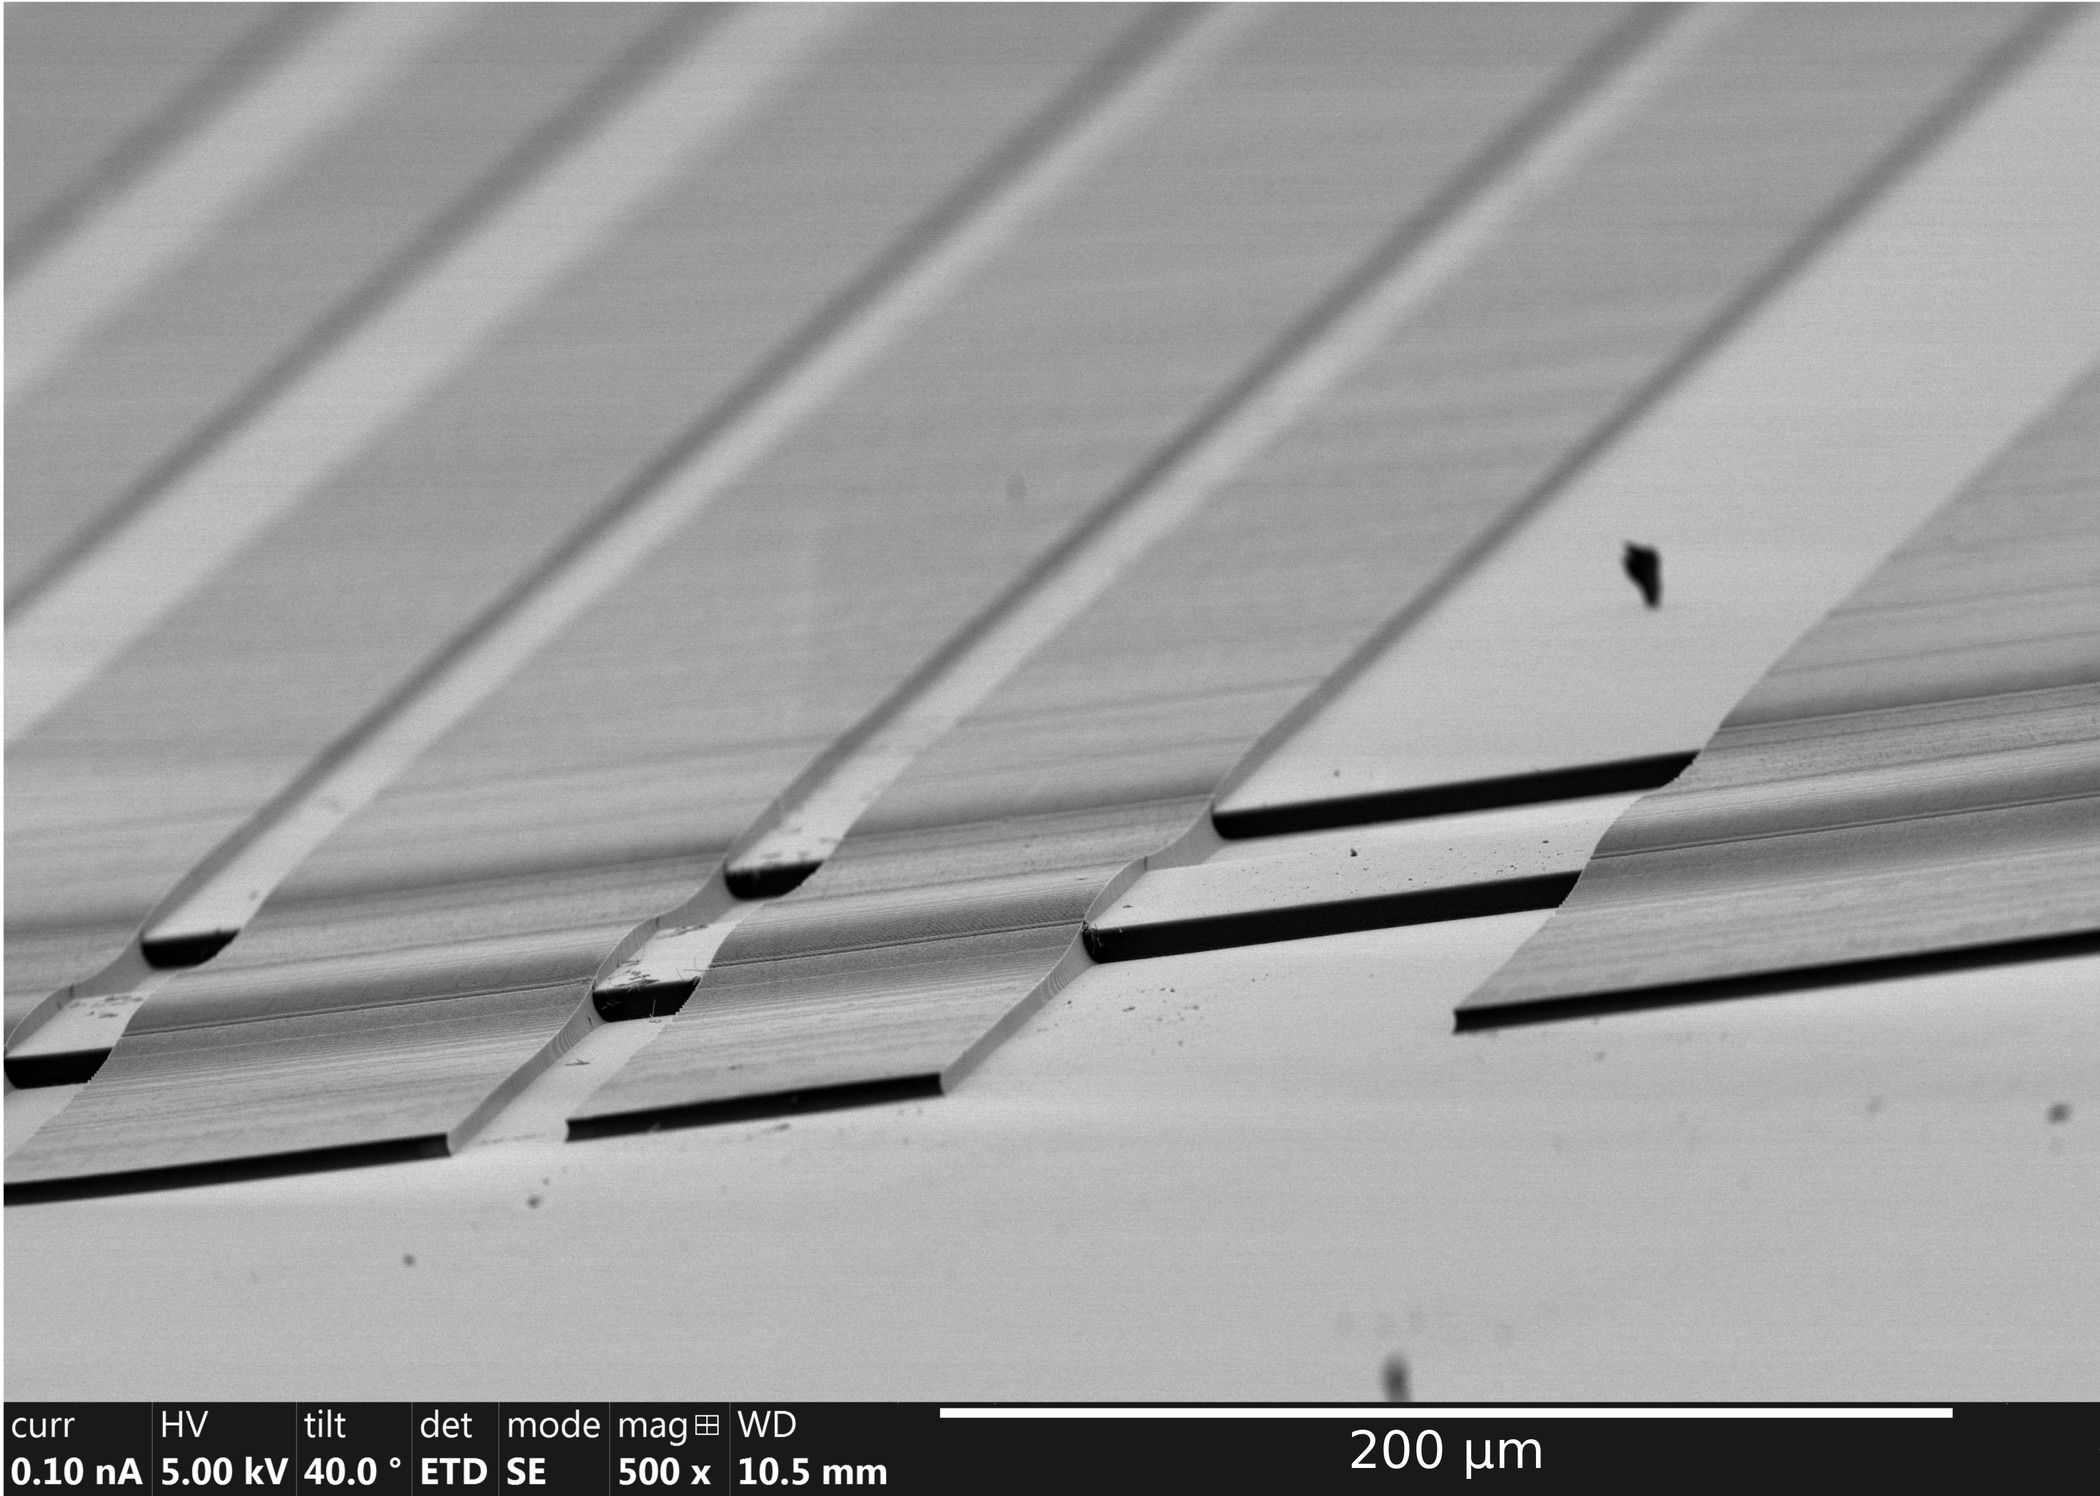
\includegraphics[width=\linewidth]{fig/mr-DWL/sem_mr-dwl-2.jpg}
  %\caption{1a}
  \label{fig:sfig1}
\end{subfigure}% %blank line makes figures vertical

\begin{subfigure}{.5\textwidth}
  \centering
  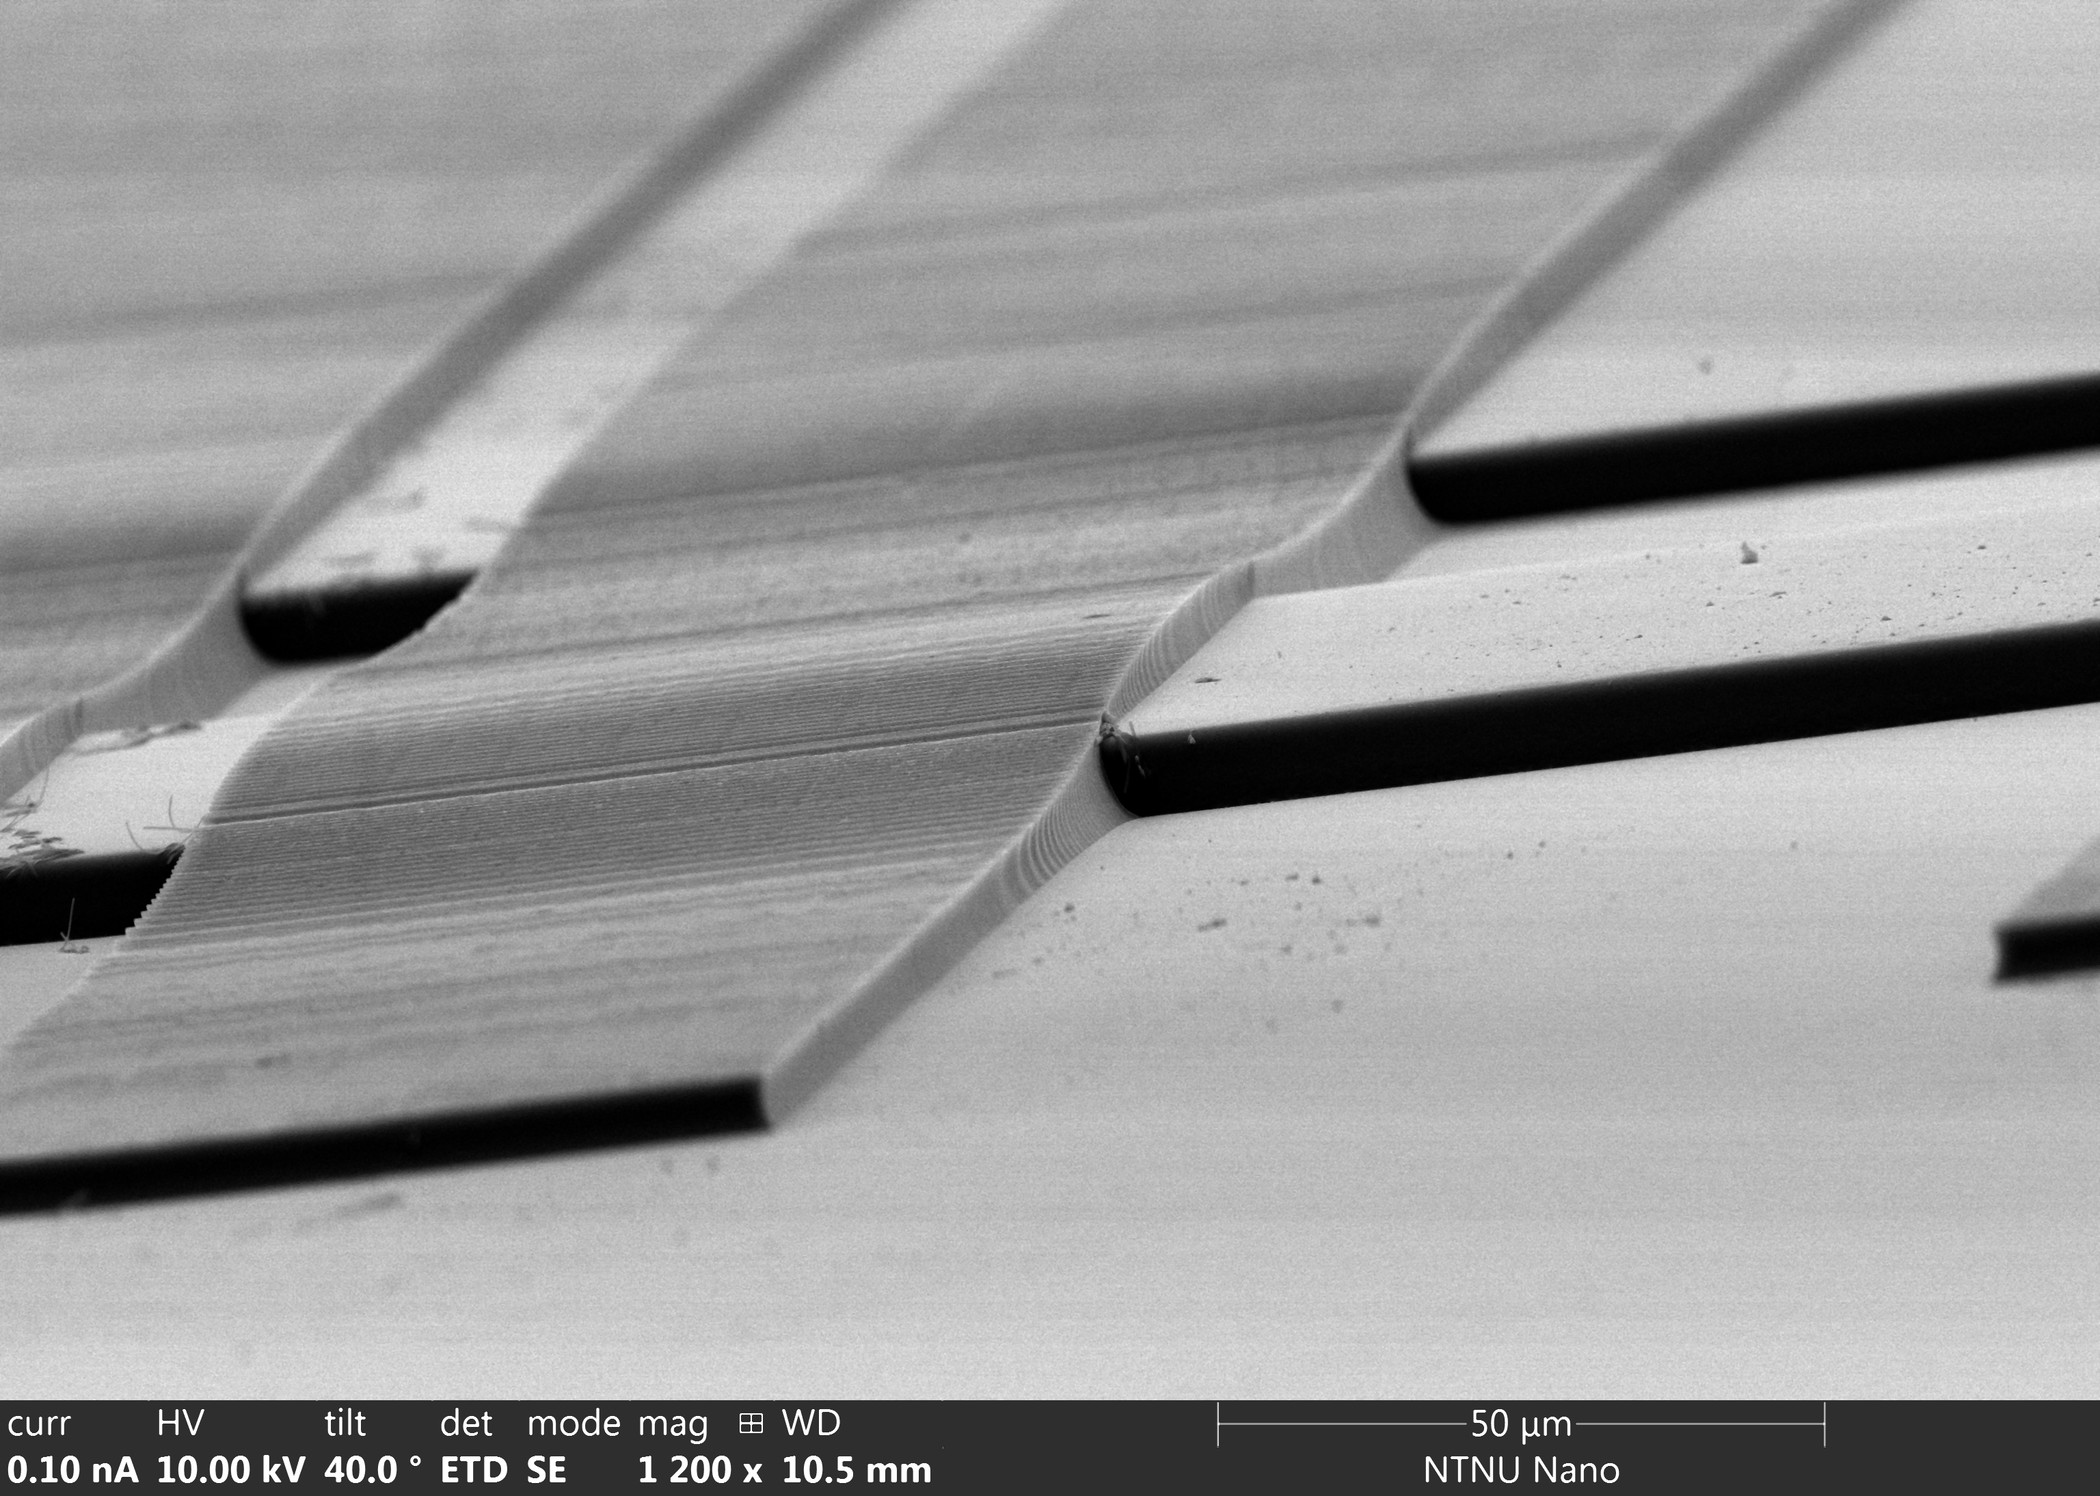
\includegraphics[width=\linewidth]{fig/mr-DWL/sem_mr-dwl.jpg}
  %\caption{1b}
  \label{fig:sfig2}
\end{subfigure}
\caption{$5um$ mr-DWL resist structures coated with a $4um$ man440 layer, demonstrating the possibility of patterning resist structures over a high step edge. }
\label{fig:fig}
\end{wrapfigure}

A remaining problem with the sample preparation is cracking in the glass cladding that impedes the path of the electrical contacts. This consistently happens with a parallel crack propagating on at least one side of the core. It becomes more severe in samples with a larger core to cladding ratio, and in hand drawn samples. Not only does this limit the contact spacing and the number of measurements that can be done on one sample, it aso affects the ability to make hall measurements, as the hall pattern requires contacts on either side of the fiber. It is sometimes the case that only a small amount of a particular sample is drawn, and then each sample becomes more important, and a failure during preparation will set back the work significantly. This is the case if we desire to write structures within the fiber and examine this particular point. Due to the small size of the cracks, it is unlikely that filling them with a method such as vacuum impregnation with epoxy would be successful. Further this would require a second polishing step to remove this layer from the core for electrical measurements.

While photo resist is mainly used for masking purposes, adding a permanent layer of resist would create a smooth surface without coating the core, and has the advantage of integrating easily with the current process. A second lithography step would add little to the preparation time. The challenges are that the resist layer must be stable in solvent during a second liftoff process, and that the subsequent thin film can create continuous coverage of the resist step edge. For the latter a positive resist would be the ideal choice due to the positive sidewall profile. Further a greyscale resist such ma-p1275g  would allow thick films (~100 um) and a controllable positive sidewall profile. While ma-p1275G would be an ideal choice, tests showed that it was not significantly cross linked after hard baking to withstand an acetone bath. 

The negative photo resists $SU-8$ and $mr_DWL$ are epoxy based and designed for creating high aspect ratio structures with nearly vertical sidewalls. Further a hardbake step up to 140C creates a very stable resist. While the sidewall profile is still negative, tilting the sample during depostion, or using sputtering may allow sufficient step coverage to create a continuous contact. 



A test sample using mr-DWL 5 was patterned on a Si wafer using the following parameters: spin 3000 patterning $500 mj/cm^2$ $405nm$ in MLA hard bake 30 min $140C$. This structure was then coated with a layer of man-440 



\section{Mrdwl on a Fiber}
The procedure was tested on a fiber to examine how the process would work under practical conditions, as the resist thickness, bake temperature and reflections during exposure would all be slightly effected. 



\begin{figure}[h]
 %h here H requires float, exactly here, h! overide latex
\centering
\begin{subfigure}{\textwidth}
  \centering
  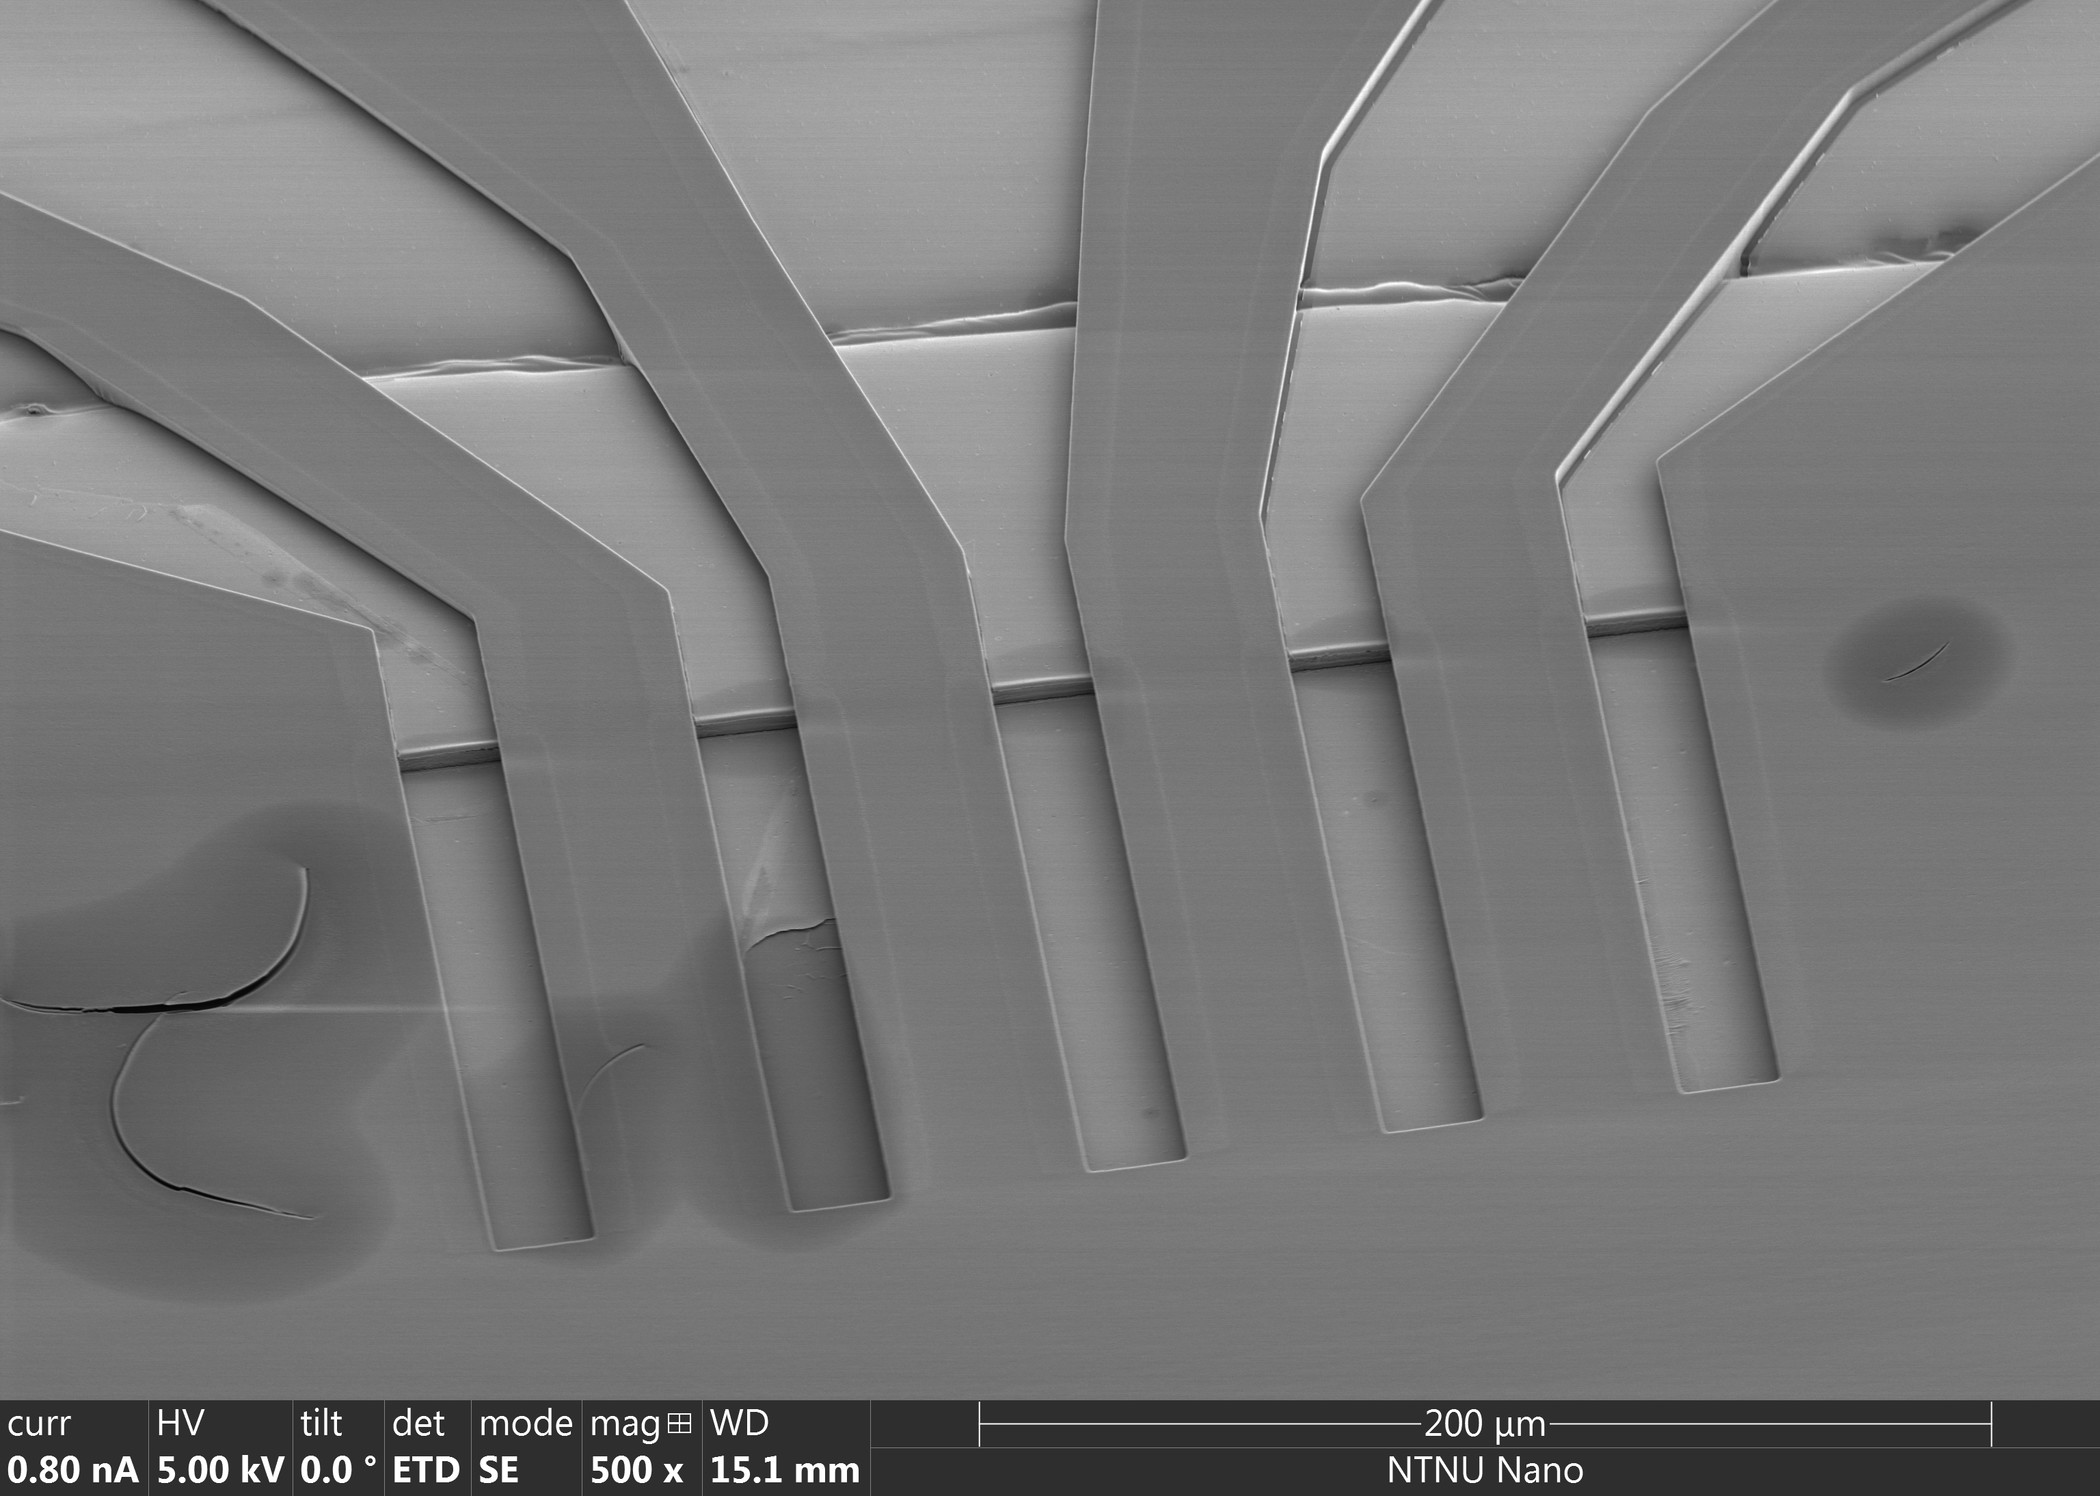
\includegraphics[width=\linewidth]{fig/mr-DWL/mb_25_overview_002.jpg}
  %\caption{1a}
  \label{fig:sfig1}
\end{subfigure}% %blank line makes figures vertical

\begin{subfigure}{\textwidth}
  \centering
  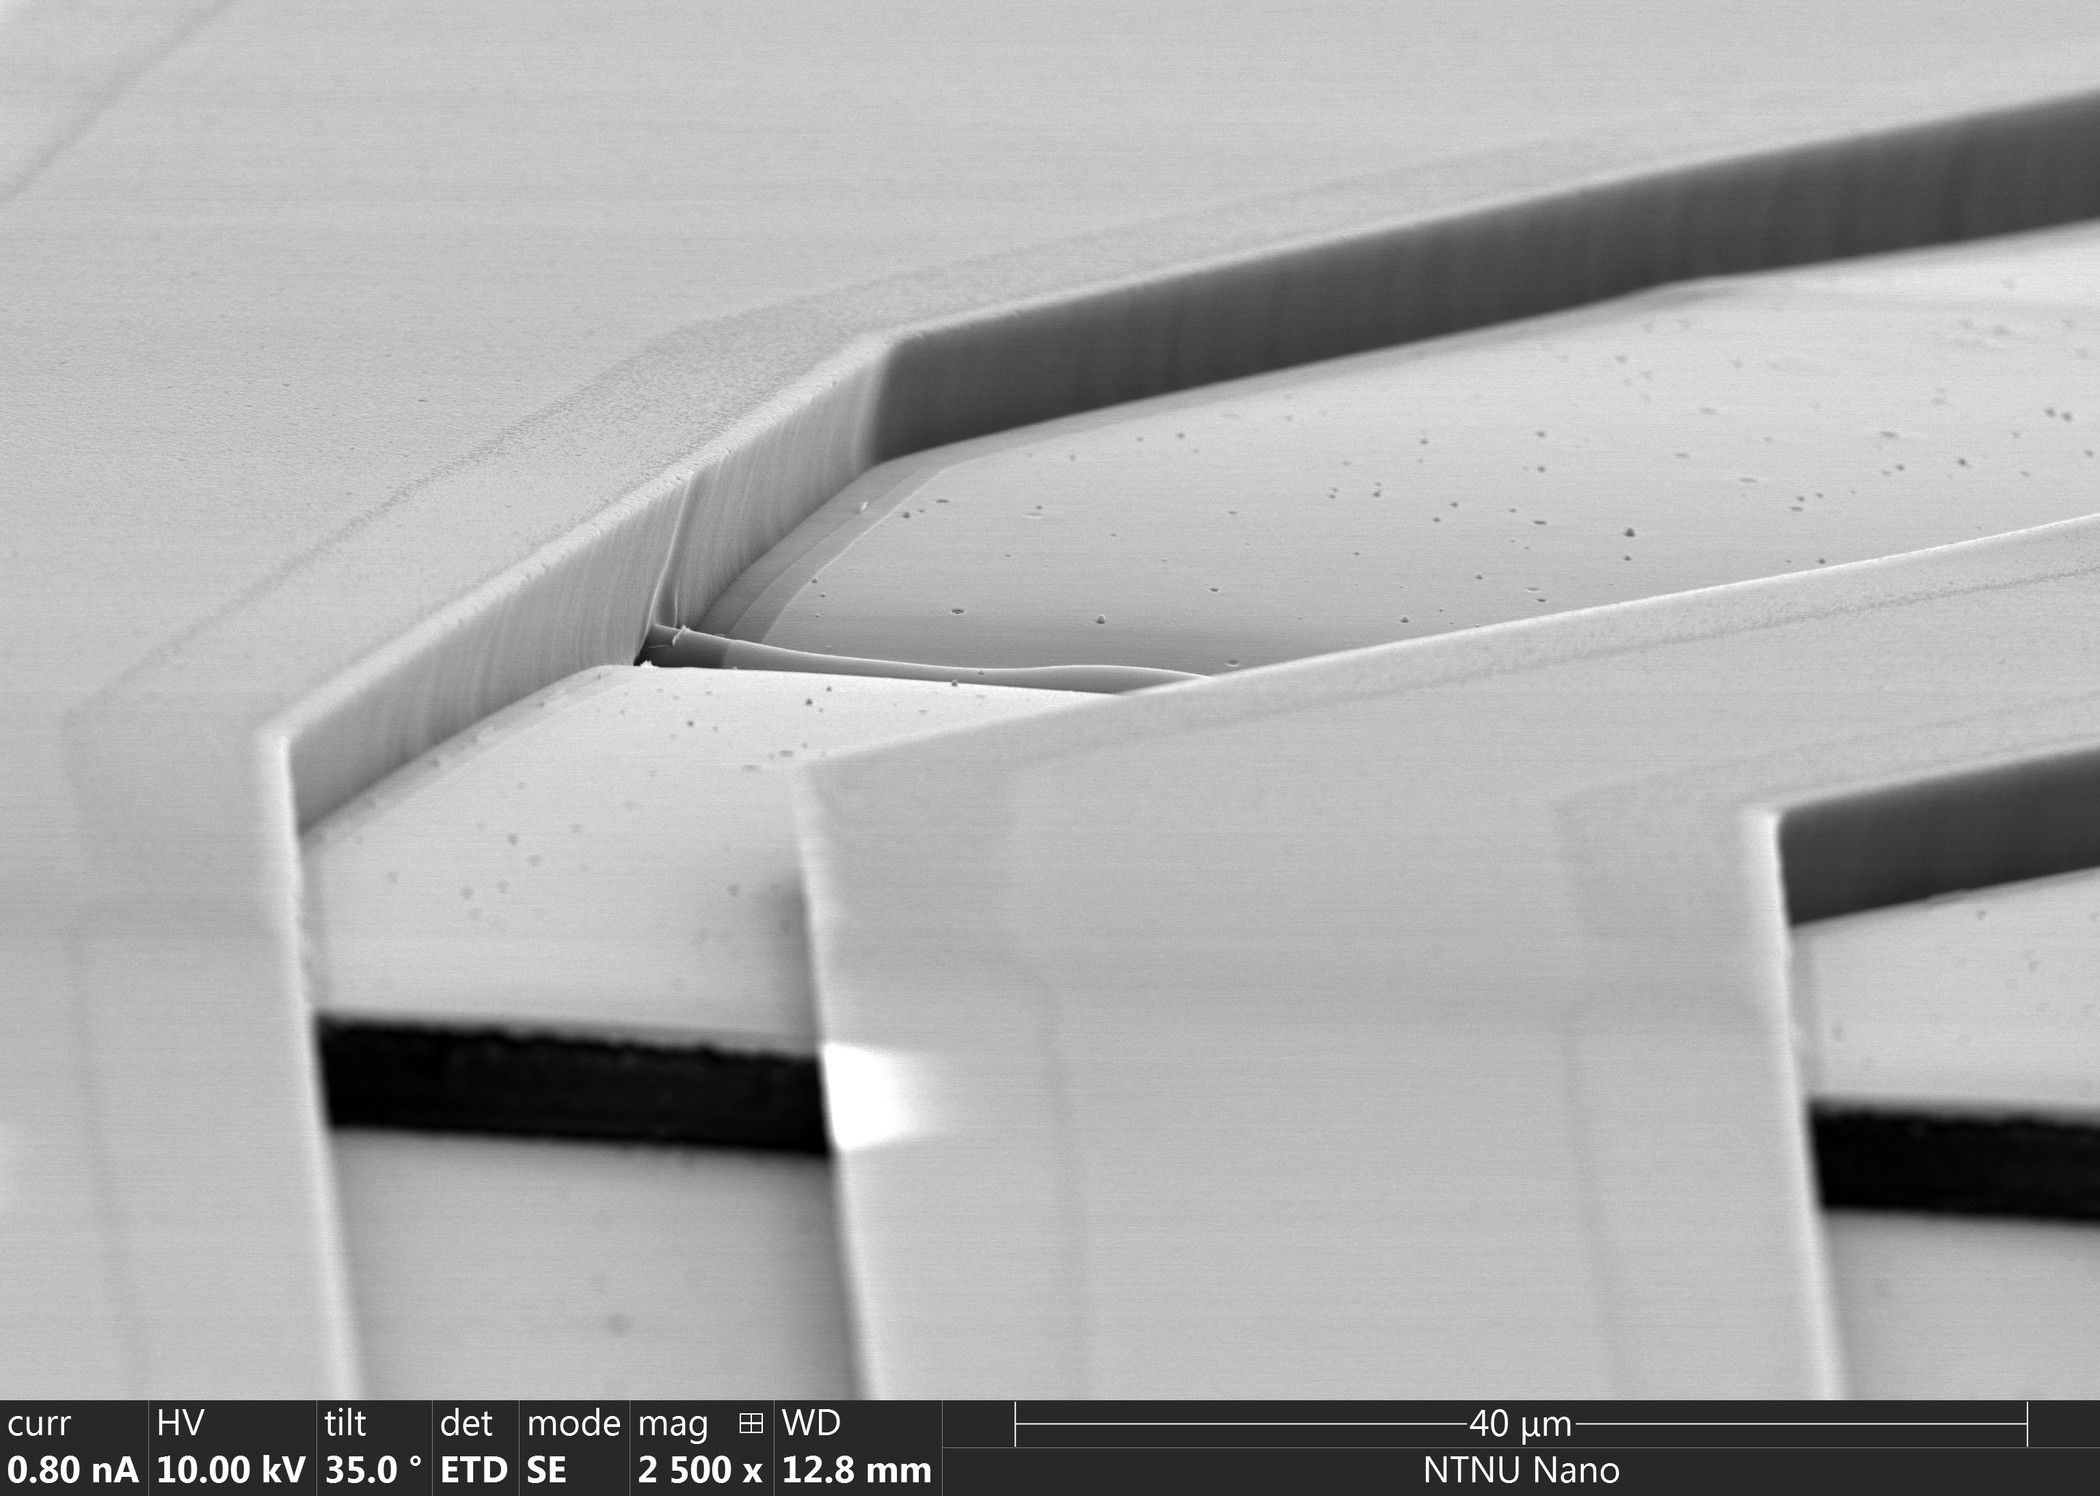
\includegraphics[width=\linewidth]{fig/mr-DWL/mb_25_step_004.jpg}
  %\caption{1a}
  \label{fig:sfig2}
\end{subfigure}% %blank line makes figures vertical

\caption{}
\label{fig:si_sige}
\end{figure}


\begin{figure}[h]
 %h here H requires float, exactly here, h! overide latex
\centering
\begin{subfigure}{\textwidth}
  \centering
  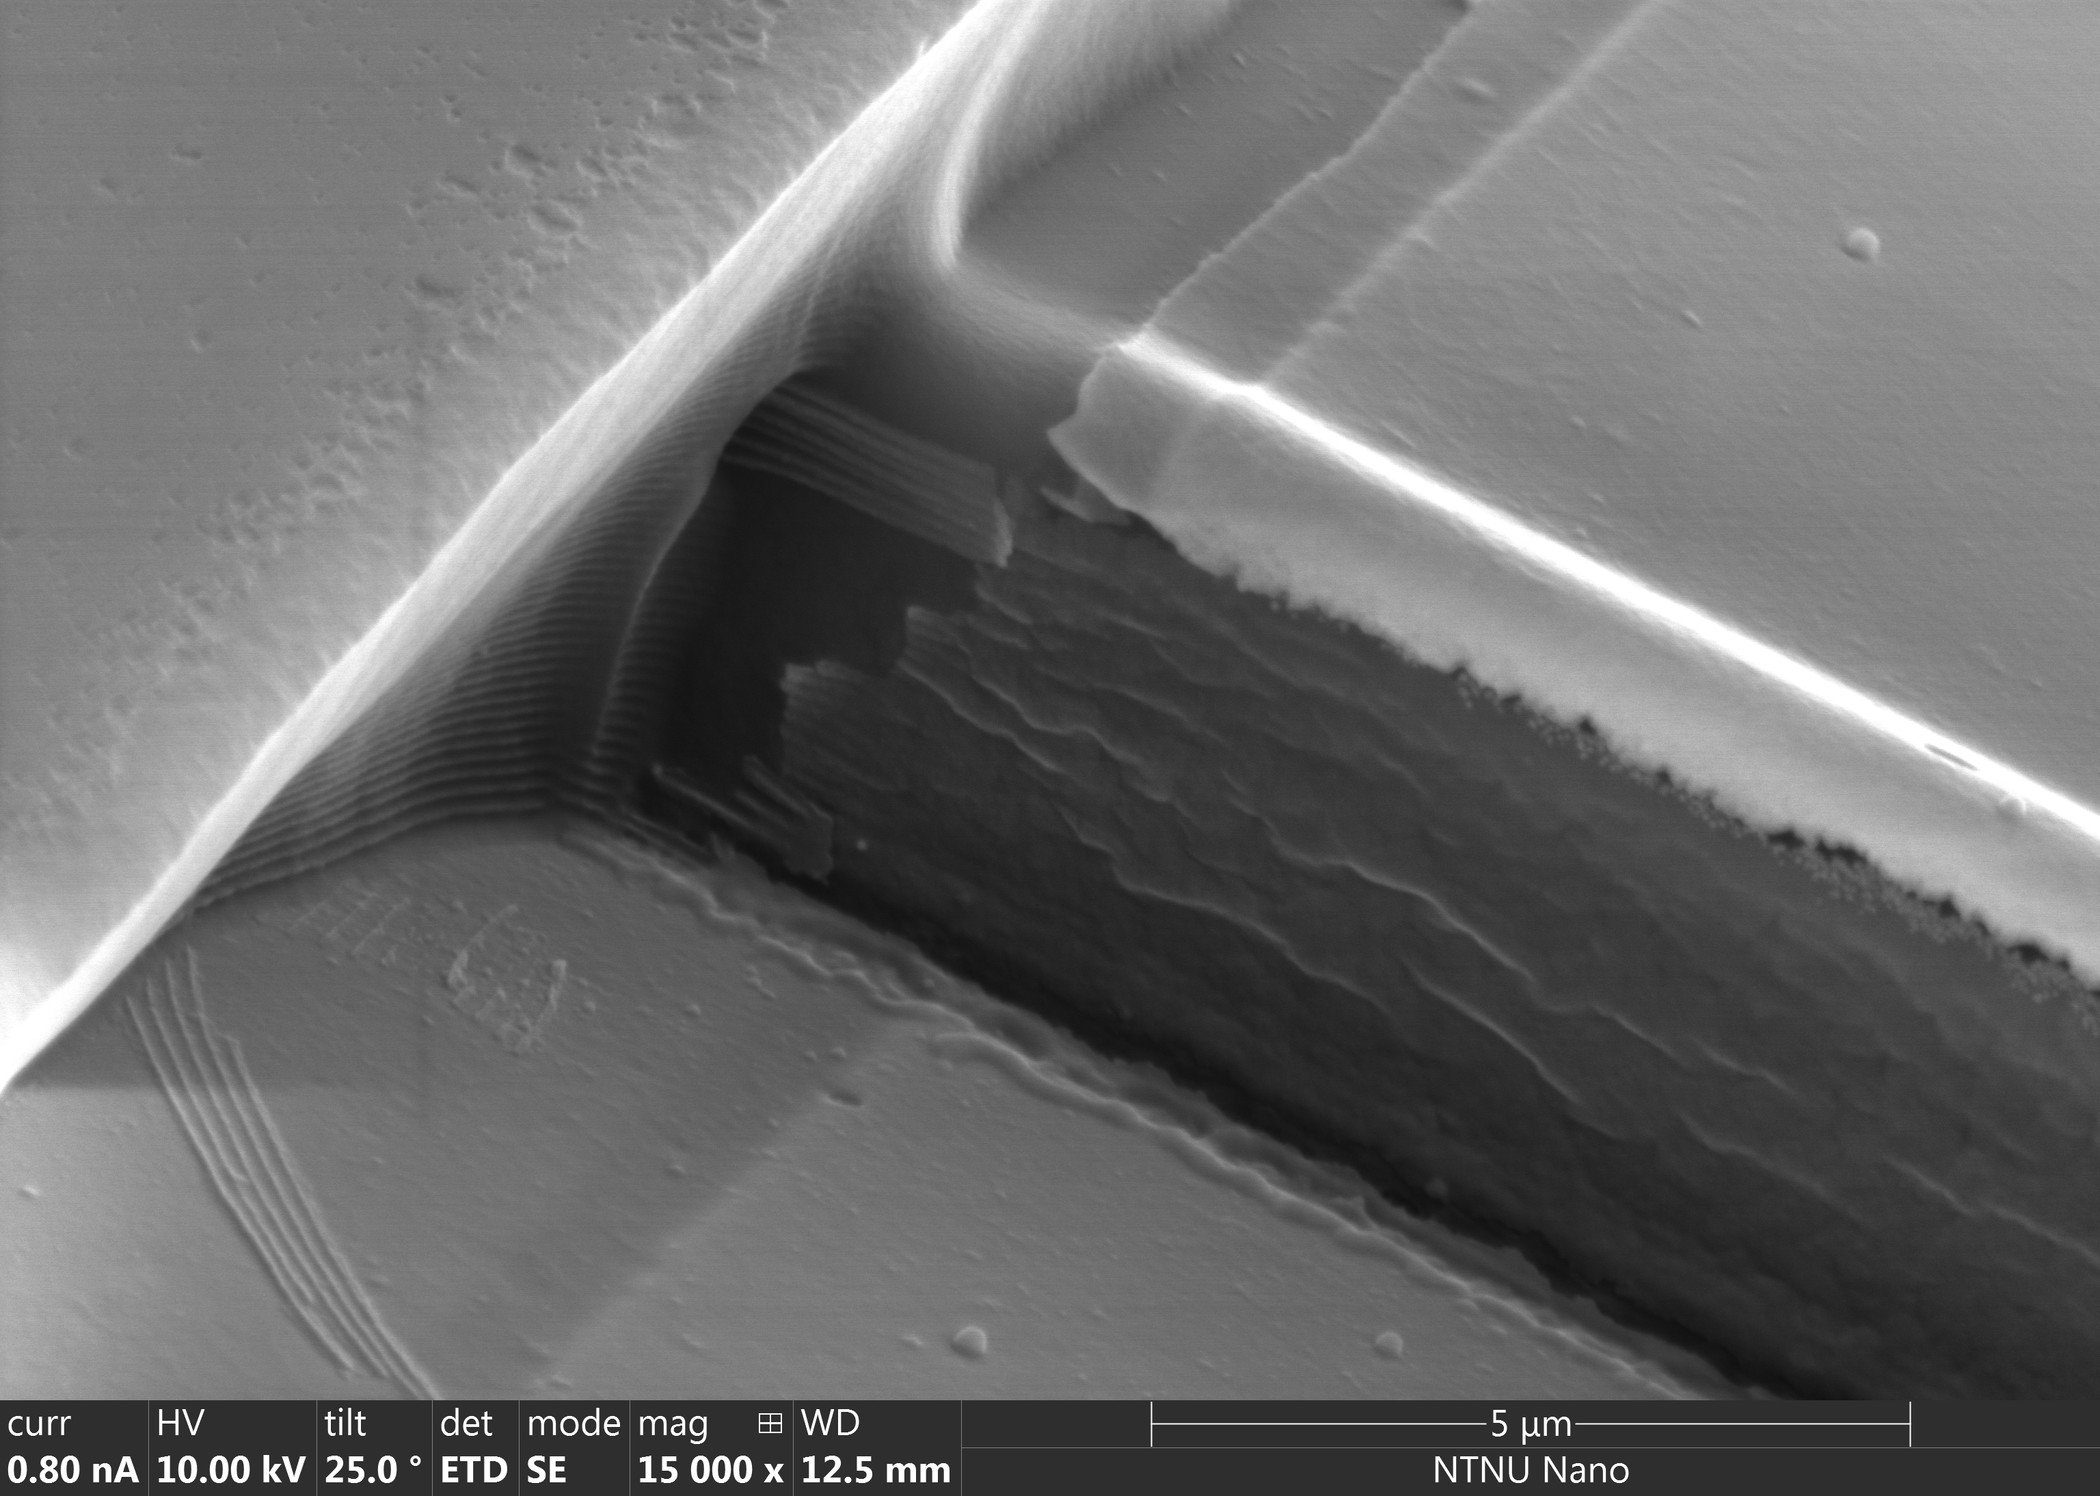
\includegraphics[width=\linewidth]{fig/mr-DWL/mb_25_step_close1.jpg}
  %\caption{1a}
  \label{fig:sfig1}
\end{subfigure}% %blank line makes figures vertical


\caption{}
\label{fig:si_sige}
\end{figure}


\begin{figure}[h]
    \centering
    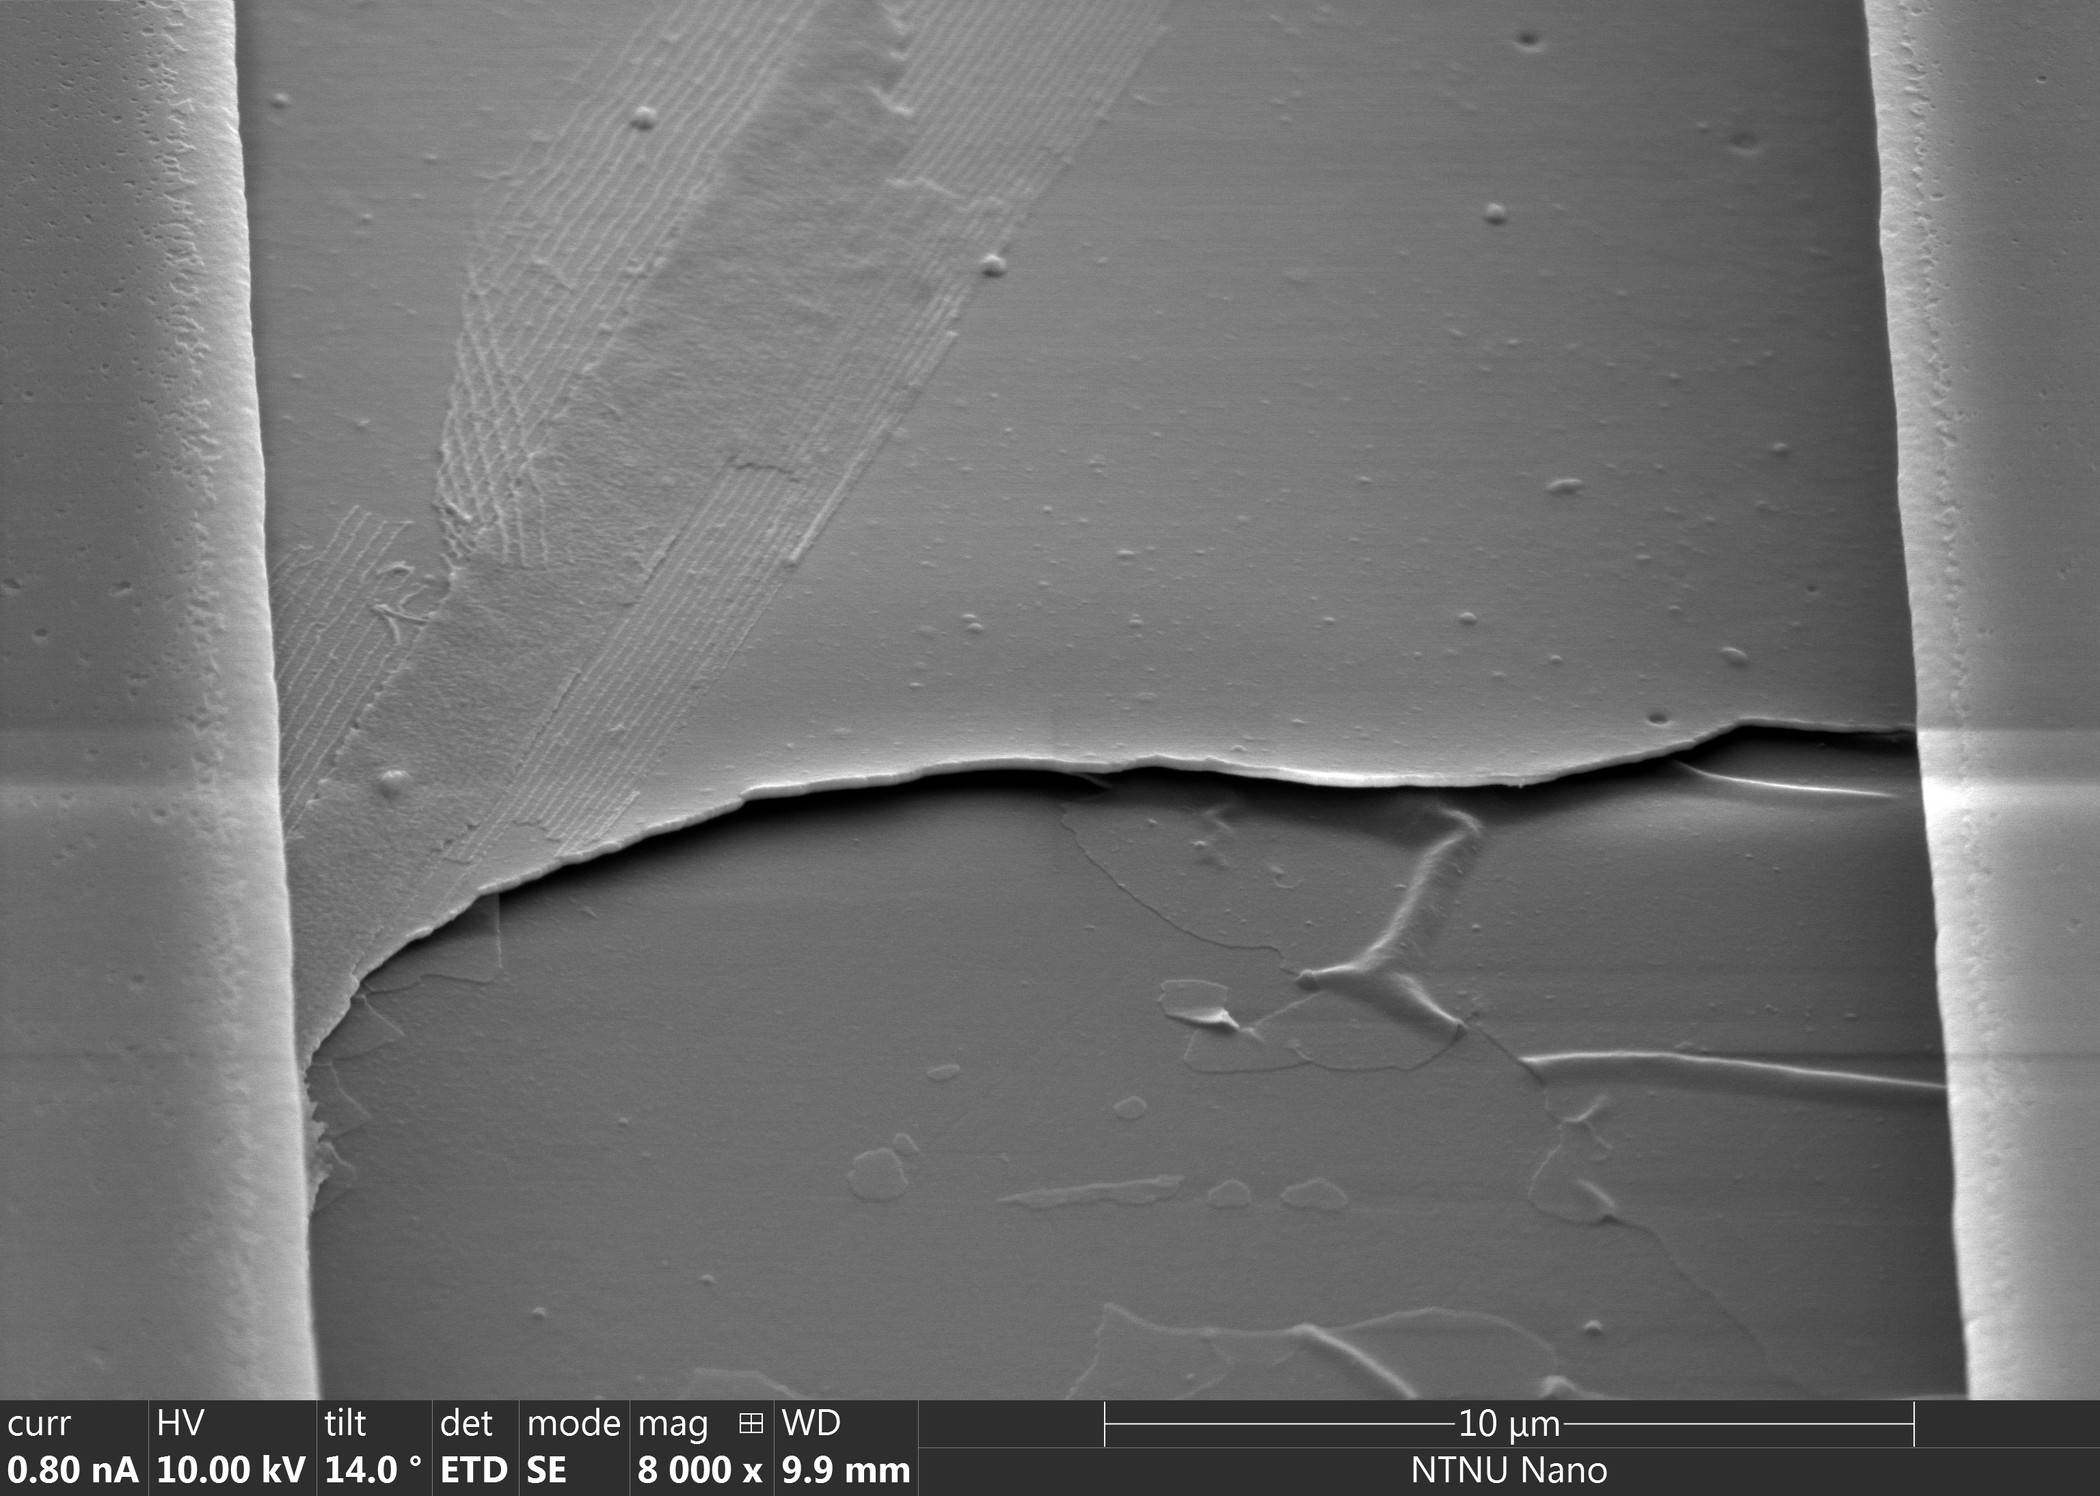
\includegraphics[width=\textwidth]{fig/mr-DWL/mb_25_step_002.jpg}
    \caption{Caption}
    \label{fig:my_label}
\end{figure}

\cleardoublepage